\documentclass{cernatsnote}
\usepackage[colorinlistoftodos]{todonotes}
\usepackage{placeins}
% \usepackage[pdftex]{graphicx}
\usepackage{smartdiagram}
\usesmartdiagramlibrary{additions}
\usepackage[capitalise]{cleveref}
\usepackage{booktabs}
\usepackage{xspace,upgreek}
\usepackage{units_definitions}
\usepackage{tikz}
\usepackage{subfig}
\usepackage{amsmath}


\title{Simulation studies for a drift chamber at the FCC-ee experiment}
\author{
	Niloufar Alipour Tehrani \; \\
	CERN, CH-1211 Geneva, Switzerland
}
\email{niloufar.alipour.tehrani@cern.ch}
\date{\today}

\begin{document}
\maketitle

\begin{abstract}
	The physics aims at the electron-positron option for  the Future Circular Collider (FCC-ee)~\cite{Gomez-Ceballos:2013zzn}, impose high precision requirements on the vertex and tracking detectors.  The detector has also to match the experimental conditions such as the collisions rate and the presence of beam-induced backgrounds.
	A light weight tracking detector is under investigation for the IDEA (International Detector for Electron-Positron Accelerator) detector concept and consists of a drift chamber. Simulation studies of the drift chamber using the FCCSW (FCC software) are presented. Full simulations are used to study the effect of beam-induced backgrounds on this detector.
\end{abstract}
\\ \\ \\

\begingroup
\color{black}
\tableofcontents
\endgroup

\pagebreak

\section{Introduction}
The FCC-ee high-luminosity circular electron-positron collider, with center-of-mass energies $\sqrt{s}$ from $91.2\,\gev$ to
$365\,\gev$, allows for high-precision measurements of the properties of the Z, the W, the top quark and the Higgs boson. As a predecessor of a new $100\,\tev$ proton-proton collider, the FCC-ee collider is foreseen to be placed in a 100~km tunnel in Geneva area as shown in~\cref{fig_fcc_cern}.

\begin{figure}[ht]
	\centering
	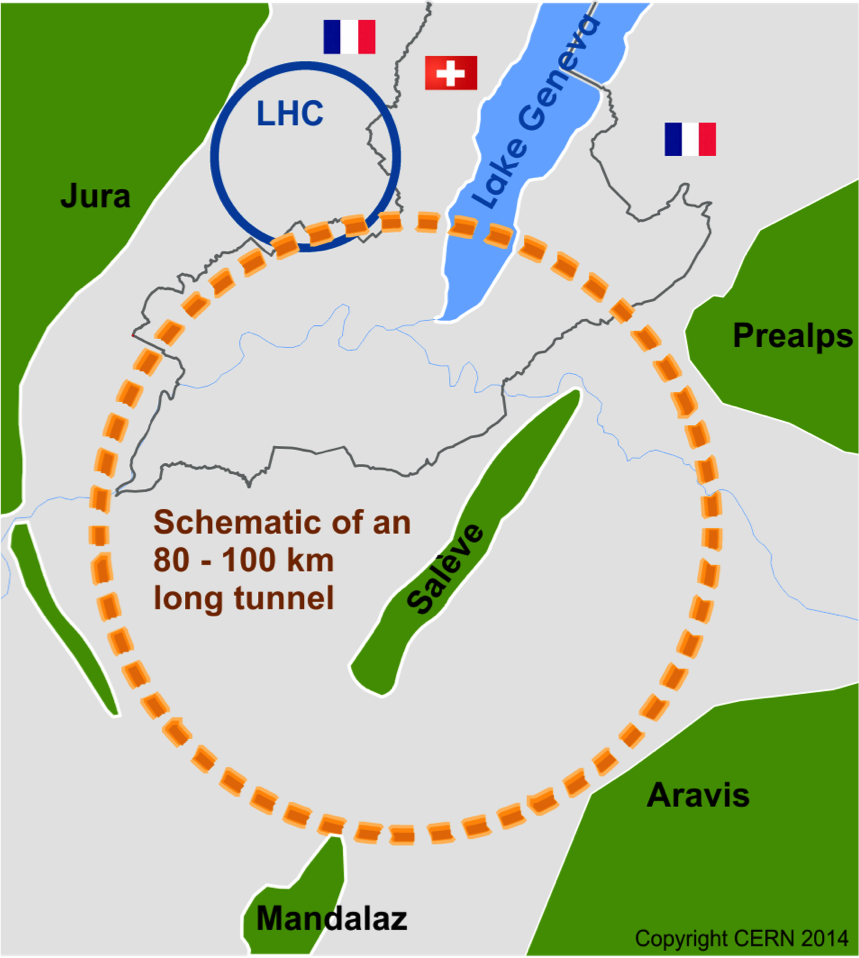
\includegraphics[width=0.8\textwidth]{figures/cernFCC.jpg}%
	\caption{A possible realization of the FCC experiment near the Geneva region.}
	\label{fig_fcc_cern}
\end{figure}

The IDEA detector, one of the two detector concepts under development for FCC-ee, has demanding requirements to match the experimental conditions. Its main components consist of: an ultra-light silicon-based vertex detector, an ultra-light drift chamber for track reconstruction and particle identification, a dual-readout calorimeter, a 2~T axial magnetic field and an instrumented return yoke as illustrated in~\cref{fig_IDEA}. The drift chamber is being investigated using \textsc{Geant4}-based simulations. Its performance and the effect of beam-induced backgrounds are presented here-below.

\begin{figure}[ht]
	\centering
	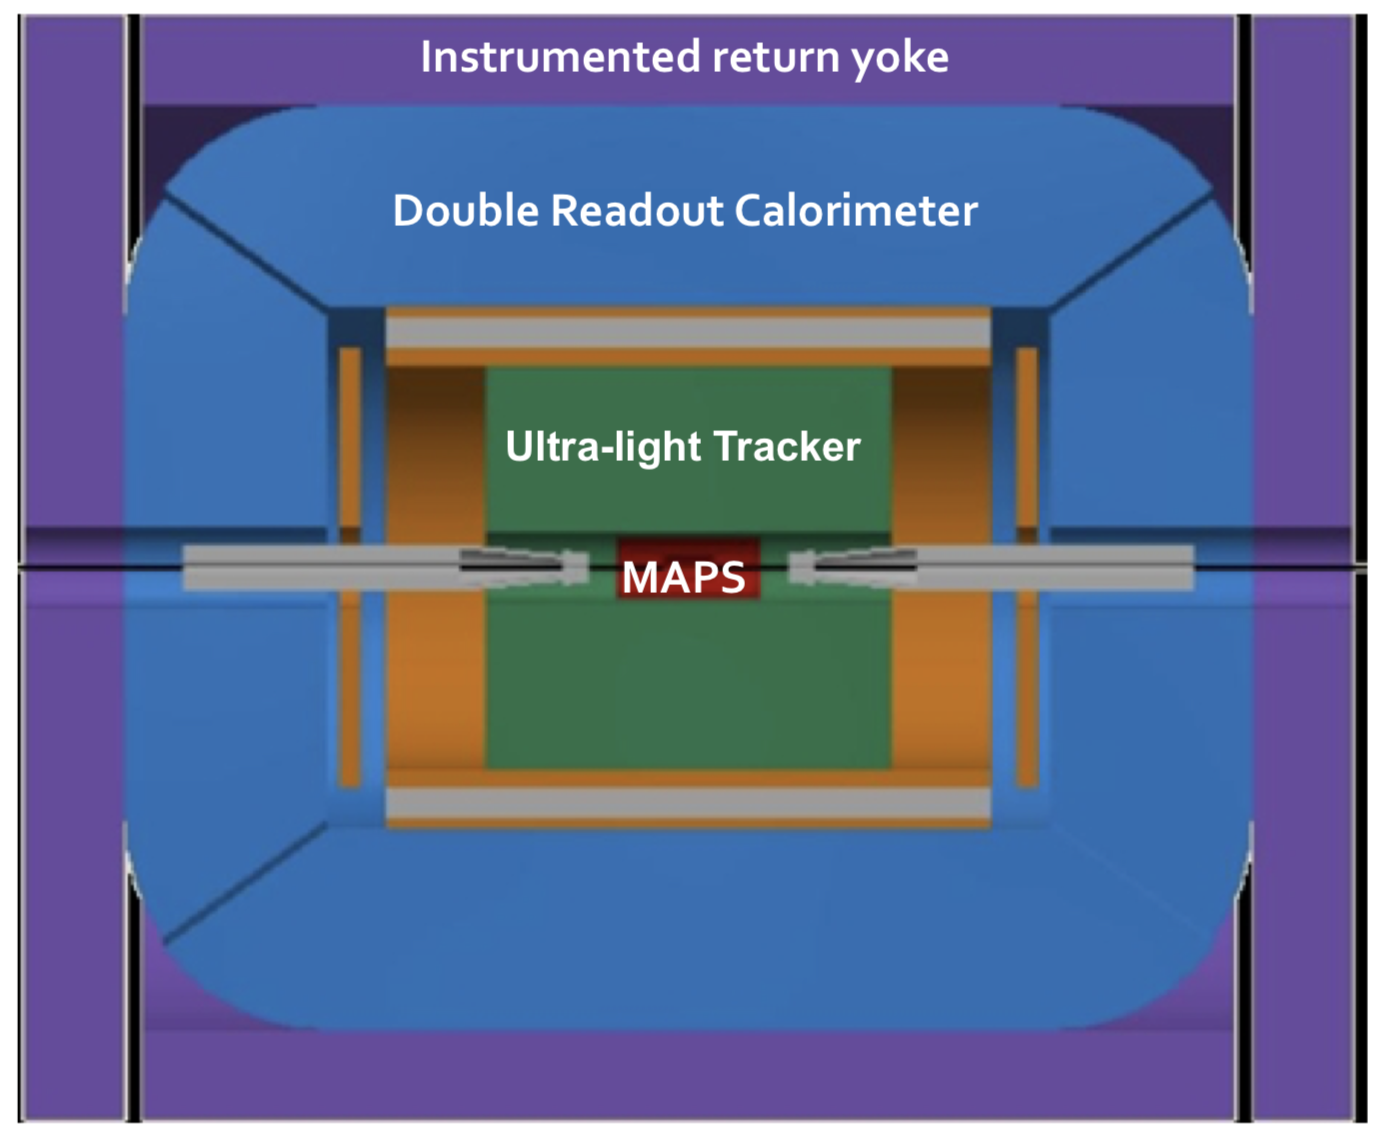
\includegraphics[width=0.8\textwidth]{figures/FCCeeIDEAConcept}%
	\caption{Schematic layout of the IDEA detector with the sub-detectors illustrated in different colors: vertex detector (red), drift chamber (green), pre-shower (orange), magnet (gray), calorimeter (blue), magnet yoke and muon system (violet).}
	\label{fig_IDEA}
\end{figure}



\section{Tracking}

The drift chamber, with 112 layers of wires, provides high number of measurements which can be exploited for the track reconstruction.

One of the methods we are investigated is the Hough transform as described below.

\subsection{The Hough Transform}
Initially invented for bubble chamber photographs~\cite{HTWikipedia}, the Hough Transform is a feature extraction technique used in several fields such as image analysis, computer vision and digital image procession. It allows for the identification of lines as well as other shapes such as circles or ellipses.

\subsubsection{Principle}
The simplest case of Hough transform is detecting straight lines. In the parameter space, lines are represented as a point (b, m) with \cref{lineeq}.

\begin{equation}
	y = m \cdot x + b
	\label{lineeq}
\end{equation}

\begin{figure}[ht]
	\begin{tikzpicture}[scale=1.5]
    % Draw axes
    \draw [<->,thick] (0,2) node (yaxis) [above] {$y$}
        |- (3,0) node (xaxis) [right] {$x$};
    % Draw two intersecting lines
    \draw (0,0) coordinate (a_1) -- (2, 2) coordinate (a_2);
    \draw (0,1.5) coordinate (b_1) -- (1.8,0) coordinate (b_2);

    \coordinate (c) at (intersection of a_1--a_2 and b_1--b_2);
		% right angle
    \fill[red] (c) circle (2pt);

\end{tikzpicture}
\caption{TODO: A line is representate as a point (b, m) in the parameter space according to \cref{lineeq}.}
\label{fig_lineParamSpace}
\end{figure}

With the presentation (b, m) in the parameter space, vertical lines pose problems for the unbounded slope parameter \textit{m}. The Hesse normal form as described in \cref{line_hesse} can be used as a solution to get around vertical lines, where $r$ is the shortest distance from the origin to the line and $\theta$ is the angle between the $x$ axis and the line connecting the origin with the closest point as illustrated in \cref{fig_lineParamSpace}. The (r, $\theta$) plane is referred to as the Hough Space.


\begin{equation}
	r = x \cdot \cos(\theta) + y \cdot \sin(\theta)
	\label{line_hesse}
\end{equation}

% \begin{figure}[ht]
% 	\centering
% 	\begin{subfigure}[b]{0.5\textwidth}
%         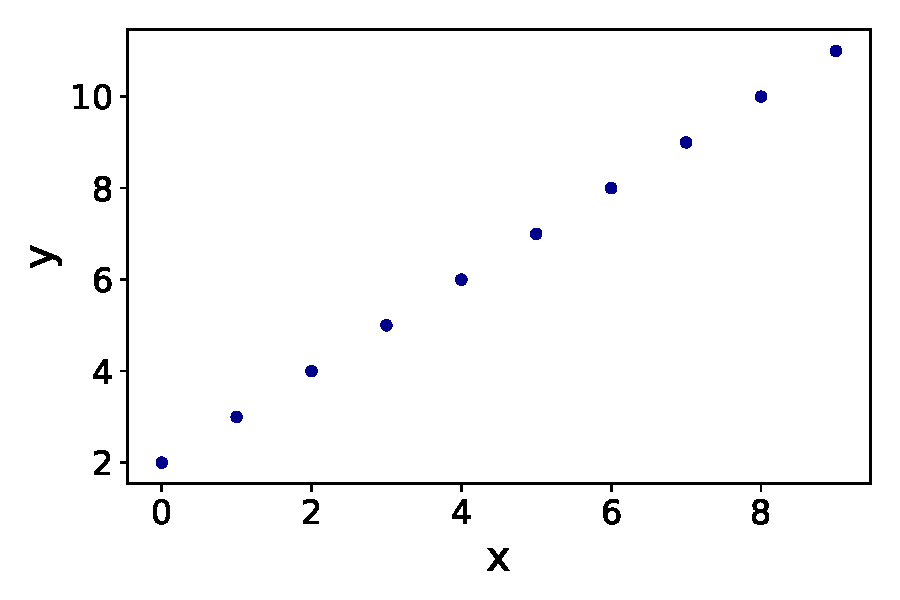
\includegraphics[width=0.8\textwidth]{figures/line.pdf}
%         \caption{A gull}
%         \label{pointsLine}
%     \end{subfigure}~
% 		\begin{subfigure}[b]{0.5\textwidth}
% 					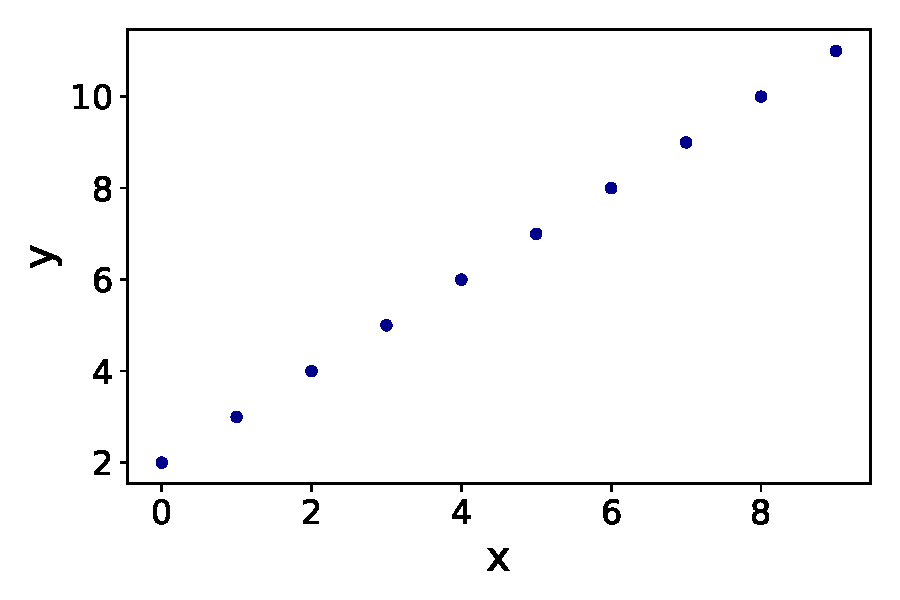
\includegraphics[width=0.8\textwidth]{figures/line.pdf}
% 					\caption{A gull}
% 					\label{pointsLine}
% 			\end{subfigure}
% \caption{\label{fig:StandardMagnetLayout} Standard magnet layout for a sector bending magnet}
% \end{figure}


\bibliography{references}
\bibliographystyle{plain}

\end{document}
